
%%%%%%%%%%%%%%%%%%%%%%%%%%%%%%%%%%%%%%%%%%%%%%%%%%%%%%%%%%%%%%%%%%%%%%
\section{Risk Informed Credibility Plan }

As outlined in ASME V\&V 40, a risk-informed approach to model credibility requires clear definition of the question of interest, context of use, and associated model risk. These three elements guide the rigor required for each credibility activity.

\paragraph{Question of Interest:} What are the potential bioeffects resulting from chemical deposition onto the oral mucosa in users of an Electronic Drug Delivery System (EDDS)?

\paragraph{Context of Use:} A fluid and heat transfer model is used to characterize the velocity and temperature distribution within representative mouth cavity geometries of EDDS users. This information supports downstream chemical transport and deposition modeling.

\paragraph{Risk Assessment:} The model is assessed as having **low influence** on decision-making and a **moderate consequence** if incorrect. Based on the ASME V\&V 40 framework, this places the overall model risk between low and moderate (see Figure~\ref{fig:riskAssessment}).

\begin{figure}[H]
    \centering
    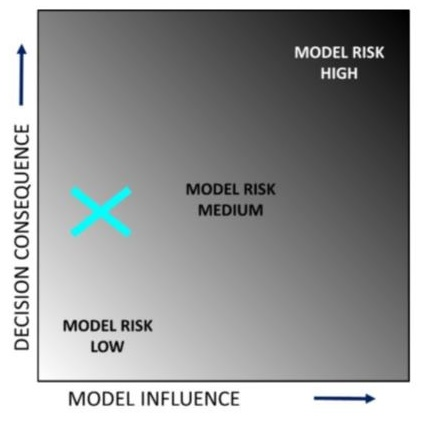
\includegraphics[width=0.5\linewidth]{figures/schematic/risk_assessment.jpg}
    \caption{Model risk classification based on decision consequence and model influence, as defined in ASME V\&V 40 \cite{vv40}.}
    \label{fig:riskAssessment}
\end{figure}

Based on this risk assessment, the required level of rigor for each credibility activity (e.g., verification, validation, uncertainty quantification) can be determined. Figure~\ref{fig:credibilityvvuq} shows the credibility activities aligned with the level of rigor gradations.

\begin{figure}[H]
    \centering
    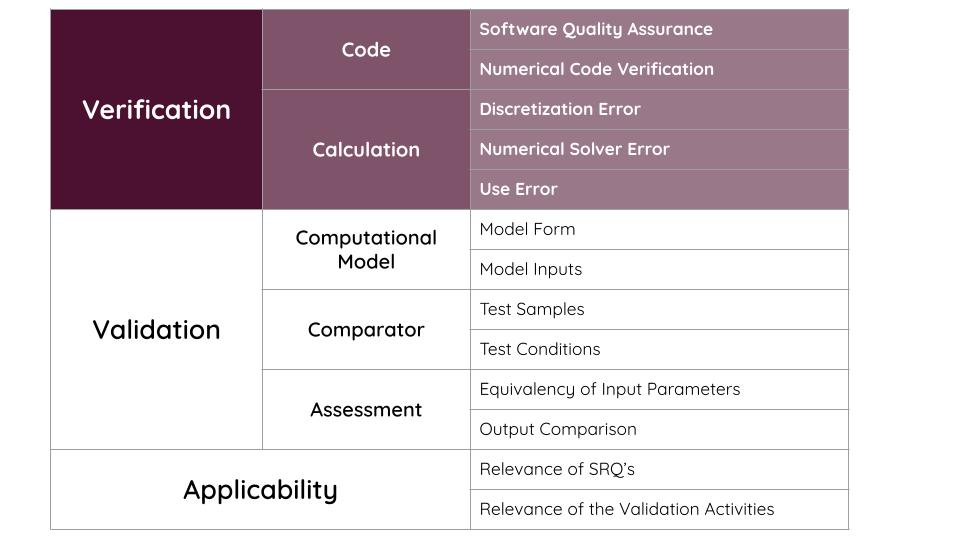
\includegraphics[width=0.8\linewidth]{figures/schematic/vvuq_workflow.jpg}
    \caption{Credibility activities and recommended rigor gradations based on model risk, following ASME V\&V 40 \cite{vv40}.}
    \label{fig:credibilityvvuq}
\end{figure}